\documentclass[11pt]{article}
\usepackage[utf8]{inputenc}
\usepackage[T1]{fontenc}
\usepackage{lmodern}
\usepackage[margin=1in]{geometry}
\usepackage{amsmath,amssymb}
\usepackage{graphicx}
\usepackage{booktabs}
\usepackage{authblk}
\usepackage[super,comma,sort&compress]{natbib}
\usepackage{xcolor}
\usepackage[colorlinks=true,allcolors=blue]{hyperref}
\usepackage{microtype}
\usepackage{caption}
\usepackage{float}
\usepackage{pifont}
\captionsetup{labelfont=bf,font=small,labelsep=period}
\renewcommand{\tablename}{Supplementary Table}
\renewcommand{\figurename}{Supplementary Fig.}

\title{\bfseries Supplementary Information for\\
``Learned variable-support priors accelerate symbolic regression of physical laws''}
\author[1]{Chenxi He\thanks{Corresponding author: \texttt{ch2067@cam.ac.uk}}}
\author[2]{Jingqiu Chen}
\affil[1]{\small Cavendish Laboratory, University of Cambridge, Cambridge CB3 0HE, United Kingdom}
\affil[2]{\small College of Physics and Optoelectronic Engineering, Shenzhen University, Shenzhen 518060, China}
\date{}

\begin{document}
\maketitle

\renewcommand{\thetable}{S\arabic{table}}
\renewcommand{\thefigure}{S\arabic{figure}}
\setcounter{table}{0}
\setcounter{figure}{0}

This Supplementary Information contains: (i) a selector-summary table that
compares DenoisedSR with five classical feature selectors across AI-Feynman,
SRSD-Feynman and noise levels (Supplementary Table~\ref{tab:selector-summary});
(ii) a threshold-sensitivity table demonstrating that the deployed $\tau=0.10$
operating point is not cherry-picked (Supplementary
Table~\ref{tab:tau-sensitivity}); (iii) an internal-validation table reporting
two additional, internally-curated suites under a different evaluation
protocol (Supplementary Table~\ref{tab:internal-validation}); (iv) a backend
integration summary (Supplementary Table~\ref{tab:backends}); (v) the master
backend $\times$ benchmark matrix (Supplementary
Table~\ref{tab:backends-3way}); (vi) an $80$-equation Feynman scale-up
(Supplementary Table~\ref{tab:n80}); (vii) controlled variable-name ablations
(Supplementary Tables~\ref{tab:name-ablation-vars} and~\ref{tab:op-sweep});
and (viii) the SRSD-Feynman per-task precision diagnostic (Supplementary
Fig.~\ref{fig:srsd-detail}). All numbers reproduce from the released
evaluation scripts at
\href{https://github.com/ChenxiHeCam/DenoisedSR}{\nolinkurl{https://github.com/ChenxiHeCam/DenoisedSR}}
(archived at
\href{https://doi.org/10.5281/zenodo.20584889}{\nolinkurl{10.5281/zenodo.20584889}}).


\begin{table}[h!]\centering
\caption{\textbf{Summary of variable-support recovery across selectors and
suites.} Variable-support recall, with the fraction of tasks on which the
selector attains \emph{perfect} recall (every true variable retained). All
selectors except DenoisedSR are run at an oracle top-$k$ budget that hands them
the true variable count for free. Recall on AI-Feynman is also reported under
relative Gaussian label noise $\eta$; entries marked --- were not part of the
noise sweep.}
\label{tab:selector-summary}
\footnotesize
\begin{tabular}{lcccccccc}
\toprule
& \multicolumn{2}{c}{AI-Feynman ($118$)} & SRSD ($120$) & \multicolumn{5}{c}{AI-Feynman recall under noise $\eta$} \\
\cmidrule(lr){2-3}\cmidrule(lr){4-4}\cmidrule(lr){5-9}
Selector & recall & perfect \% & recall & $0.01$ & $0.05$ & $0.10$ & $0.20$ & $0.30$ \\
\midrule
Pearson $|\rho|$           & 0.768 & 45.8 & ---   & 0.772 & 0.769 & 0.771 & 0.763 & 0.768 \\
Spearman $|\rho|$          & 0.776 & 45.8 & ---   & 0.773 & 0.770 & 0.770 & 0.757 & 0.754 \\
mutual information         & 0.634 & 20.3 & ---   & 0.633 & 0.636 & 0.644 & 0.608 & 0.605 \\
random-forest importance   & 0.812 & 44.9 & ---   & 0.815 & 0.822 & 0.815 & 0.807 & 0.799 \\
Lasso (CV) \emph{oracle $k$} & 0.905 & 71.2 & 0.723 & 0.904 & 0.904 & 0.886 & 0.881 & 0.868 \\
\midrule
DenoisedSR (ours, $\tau{=}0.10$) & \textbf{1.000} & \textbf{100.0} & \textbf{0.967} & \textbf{1.000} & \textbf{1.000} & \textbf{1.000} & \textbf{1.000} & \textbf{1.000} \\
\bottomrule
\end{tabular}
\end{table}

\begin{table}[h!]\centering
\caption{\textbf{Threshold sensitivity of the deployed RF+GAT ensemble.} Sweep
of $\tau$ on AI-Feynman ($118$ laws, $q=100$, $20$ distractors). Recall remains
$1.000$ with $100\%$ perfect-recall over $\tau\in[0.05, 0.30]$ (a sixfold range);
only at $\tau\geq 0.50$ does recall start to decline. The deployed
$\tau=0.10$ is not cherry-picked.}
\label{tab:tau-sensitivity}
\footnotesize
\begin{tabular}{ccccc}
\toprule
$\tau$ & Recall & Precision & Perfect-recall (\%) & Mean kept columns \\
\midrule
0.05 & 1.000 & 0.705 & 100.0 & 9.03 \\
0.08 & 1.000 & 0.740 & 100.0 & 8.81 \\
\textbf{0.10 (deployed)} & \textbf{1.000} & \textbf{0.749} & \textbf{100.0} & \textbf{8.76} \\
0.15 & 1.000 & 0.766 & 100.0 & 8.67 \\
0.20 & 1.000 & 0.769 & 100.0 & 8.66 \\
0.30 & 1.000 & 0.780 & 100.0 & 8.60 \\
0.50 & 0.998 & 0.873 &  99.2 & 6.31 \\
0.75 & 0.981 & 0.991 &  93.2 & 3.87 \\
1.00 & 0.959 & 1.000 &  86.4 & 3.72 \\
\bottomrule
\end{tabular}
\end{table}

\begin{table}[h!]\centering
\caption{\textbf{Internal validation under a different protocol (not directly
comparable to the four external benchmarks of Fig.~\ref{fig:recall}).}
Evaluated on internally-curated physical-law records drawn from the same
knowledge graph as the training pool, using each record's pre-sampled
observation values rather than freshly sampled tables, and without random
distractor padding. We report it as a separate scale check rather than a fifth
external suite.}
\label{tab:internal-validation}
\footnotesize
\begin{tabular}{lccc}
\toprule
Set & Equations & Recall & Perfect-recall (\%) \\
\midrule
Internal physics-law set (v5\_physics65) & 1085 & 0.999 & 99.7 \\
Internal OOD-91 curated subset           &   91 & 0.996 & 98.9 \\
\bottomrule
\end{tabular}
\end{table}

\begin{table}[h!]\centering
\caption{\textbf{Variable filter is insensitive to physical names.} Same data,
same model, same threshold $\tau=0.10$; only the variable names are changed
between ``named'' (physical: $m$, $v$, $q$, $\epsilon$, $\dots$) and
``anonymized'' ($x_0$, $x_1$, $\dots$). Across $12$ scenarios on AI-Feynman
$118$, the physical-name prior contributes at most $0.3$ percentage points of
variable filter rate. The deployed RF+GAT ensemble is dominated by the
random-forest column-statistics head; the graph-attention head's
co-occurrence-graph contribution is largely vestigial for the variable task.}
\label{tab:name-ablation-vars}
\footnotesize
\begin{tabular}{lcccccc}
\toprule
                              & \multicolumn{2}{c}{Named (physical)} & \multicolumn{2}{c}{Anonymized ($x_i$)} & \multicolumn{2}{c}{$\Delta$ (named$-$anon)} \\
\cmidrule(lr){2-3}\cmidrule(lr){4-5}\cmidrule(lr){6-7}
Scenario                      & recall & filter\% & recall & filter\% & recall & filter (pp) \\
\midrule
baseline $q{=}100$, $d{=}20$ & 1.000 & 98.4 & 0.998 & 98.3 & $+0.002$ & $+0.04$ \\
small $q{=}50$               & 1.000 & 97.0 & 0.998 & 97.0 & $+0.002$ & $+0.04$ \\
very small $q{=}20$          & 1.000 & 90.8 & 0.998 & 90.6 & $+0.002$ & $+0.18$ \\
noise $\eta=0.30$            & 1.000 & 98.7 & 0.998 & 98.6 & $+0.002$ & $+0.08$ \\
noise $\eta=0.50$            & 1.000 & 98.6 & 0.998 & 98.5 & $+0.002$ & $+0.10$ \\
noise $\eta=1.00$            & 1.000 & 98.6 & 0.998 & 98.6 & $+0.002$ & $+0.07$ \\
many distractors $d{=}50$    & 1.000 & 98.5 & 0.998 & 98.5 & $+0.002$ & $+0.04$ \\
many distractors $d{=}100$   & 1.000 & 98.6 & 0.998 & 98.5 & $+0.002$ & $+0.09$ \\
hard $q{=}20$, $\eta=0.50$   & 1.000 & 90.9 & 0.998 & 90.7 & $+0.002$ & $+0.27$ \\
\bottomrule
\end{tabular}
\end{table}

\begin{table}[h!]\centering
\caption{\textbf{Operator filter \emph{is} sensitive to physical names.}
Same data, same operator predictor, varying threshold
$\tau_{\mathrm{op}}$. Operator filter rate is the fraction of the $13$
non-trivial operators (excluding the four always-on arithmetic operators)
dropped from the search library. Physical names contribute $+7$ to $+17$
percentage points of operator recall---a much larger effect than for
variables, because the operator-vs-data signal in $(\mathbf{x},y)$ is weak and
the physics-knowledge-graph prior is the main source of information.}
\label{tab:op-sweep}
\footnotesize
\begin{tabular}{cccccccc}
\toprule
$\tau_{\mathrm{op}}$ & \multicolumn{3}{c}{Named (physical)} & \multicolumn{3}{c}{Anonymized ($x_i$)} & $\Delta$ recall \\
\cmidrule(lr){2-4}\cmidrule(lr){5-7}
 & recall & prec. & filter\% & recall & prec. & filter\% & (named$-$anon) \\
\midrule
0.03                            & 0.912 & 0.383 & 58.9 & 0.744 & 0.346 & 59.8 & $+0.168$ \\
0.10                            & 0.825 & 0.465 & 67.9 & 0.726 & 0.380 & 65.6 & $+0.099$ \\
0.20                            & 0.761 & 0.503 & 72.9 & 0.703 & 0.427 & 70.1 & $+0.058$ \\
\textbf{0.30 (deployed)}        & \textbf{0.738} & \textbf{0.536} & \textbf{76.5} & \textbf{0.667} & \textbf{0.437} & \textbf{72.9} & \textbf{$+0.071$} \\
0.50                            & 0.597 & 0.547 & 82.7 & 0.521 & 0.420 & 82.2 & $+0.076$ \\
0.70                            & 0.407 & 0.532 & 88.9 & 0.285 & 0.376 & 90.4 & $+0.122$ \\
\bottomrule
\end{tabular}
\end{table}

\begin{table}[h!]\centering
\caption{\textbf{Backend integration summary.} Mean exact-law recovery and mean
held-out $R^2$ on the $30$-equation Feynman headline subset
($n_{\mathrm{dist}}=20$, $q=100$). Errors are $\pm$s.d.\ over three random seeds.
The variable prior shrinks the candidate-column set from $23.2$ to $3.4$ in
both backends.}
\label{tab:backends}
\footnotesize
\begin{tabular}{lcc}
\toprule
Condition & Exact recovery (\%) & Mean held-out $R^2$ \\
\midrule
\multicolumn{3}{l}{\emph{PySR (10\,s budget, full $17$-op library)}} \\
\quad full search                & $42.2 \pm 13.5$ & $0.906 \pm 0.045$ \\
\quad + DenoisedSR variable prior  & $60.0 \pm 0.0$  & $0.980 \pm 0.011$ \\
\quad + DenoisedSR variable\,+\,operator prior & $60.0 \pm 11.5$ & $0.979 \pm 0.011$ \\
\midrule
\multicolumn{3}{l}{\emph{gplearn ($20$ generations, population $500$, $10$-op library)}} \\
\quad full search                & $3.3  \pm 3.3$  & $0.475 \pm 0.083$ \\
\quad + DenoisedSR variable prior  & $17.8 \pm 1.9$  & $0.763 \pm 0.029$ \\
\midrule
\multicolumn{3}{l}{\emph{PSE (parallel GPU enumeration, $30$\,s budget, $9$-op library, single seed)}} \\
\quad full search                & $0$  & $0.184$ \\
\quad + DenoisedSR variable prior  & $40$ & $0.895$ \\
\bottomrule
\end{tabular}
\end{table}

\begin{table}[h!]\centering
\caption{\textbf{Master backend $\times$ benchmark matrix.} Exact-law recovery
(\% with held-out $R^2 \ge 0.999$) on five physical-symbolic benchmarks for
three structurally different SR backends, with and without the DenoisedSR
variable prior. Cells show \emph{full backend} $\to$ \emph{+DenoisedSR}; gap in
percentage points. Multi-seed entries are mean$\pm$s.d.; single-seed entries
omit the standard deviation. PySR-Feynman118 is over three random seeds;
gplearn entries on Feynman are over three seeds; remaining cells are single
seed. PSE-SRSD is not evaluated because PSE's float32 tensor representation
underflows on SRSD's $\sim 10^{60}$-magnitude physical-unit targets (a
backend-data interaction, unrelated to the prior). Bold marks the larger of
the two values in each row.}
\label{tab:backends-3way}
\scriptsize
\setlength{\tabcolsep}{4pt}
\begin{tabular}{llccc}
\toprule
Benchmark & Distractors & PySR & gplearn & PSE \\
          &             & \emph{full} $\to$ \emph{+prior} ($\Delta$) & \emph{full} $\to$ \emph{+prior} ($\Delta$) & \emph{full} $\to$ \emph{+prior} ($\Delta$) \\
\midrule
AI-Feynman 118 (3 seeds)  & 20 random      & $46.3{\pm}3.0 \to \mathbf{57.3{\pm}1.8}$ ($\!+\!11$) & $0.8 \to \mathbf{11.0}$ ($\!+\!10$) & $8.5 \to \mathbf{42.4}$ ($\!+\!34$) \\
Strogatz 15                & 20 random      & $60.0 \to \mathbf{66.7}$ ($\!+\!7$)  & $0.0 \to 0.0$ ($0$)         & $6.7 \to \mathbf{53.3}$ ($\!+\!47$) \\
Nguyen 12                  & 20 random      & $\mathbf{91.7} \to \mathbf{91.7}$ ($0$) & $8.3 \to 8.3$ ($0$) & $33.3 \to \mathbf{100.0}$ ($\!+\!67$) \\
SRSD-Feynman 120           & ${\sim}2$ plausible & $\mathbf{54.2} \to 50.0$ ($\!-\!4$) & $30.0 \to 30.0$ ($0$) & --- \\
SRSD-Feynman 120           & + 20 random    & $42.5 \to \mathbf{54.2}$ ($\!+\!12$) & $25.0 \to \mathbf{29.2}$ ($\!+\!4$) & --- \\
\bottomrule
\end{tabular}
\end{table}

\begin{table}[h!]\centering
\caption{\textbf{Headline result scales to $80$ Feynman equations.} Repeating
the PySR comparison at the same configuration ($n_{\mathrm{dist}}=20$, $q=100$,
$\tau=0.10$, single seed) on the first $80$ Feynman tasks (chosen by
$2\le|\mathrm{features}|\le 9$) rather than the headline $30$. The gain is
preserved at larger scale; full PySR's higher absolute rate at this scale
($54\%$ vs.\ $30$--$57\%$ across seeds at $n{=}30$) is consistent with the
$30$-equation subset including a higher fraction of harder formulas.}
\label{tab:n80}
\footnotesize
\begin{tabular}{lccc}
\toprule
Condition & Exact (\%) & Mean held-out $R^2$ & Variable recall \\
\midrule
full PySR (all $23$ cols, $17$ ops)        & $54$ & $0.900$ & --- \\
+ DenoisedSR variable prior ($3.4$ cols)   & $66$ & $0.981$ & $1.000$ \\
+ DenoisedSR variable\,+\,operator prior   & $68$ & $0.981$ & $1.000$ \\
\bottomrule
\end{tabular}
\end{table}

\begin{figure}[h!]\centering
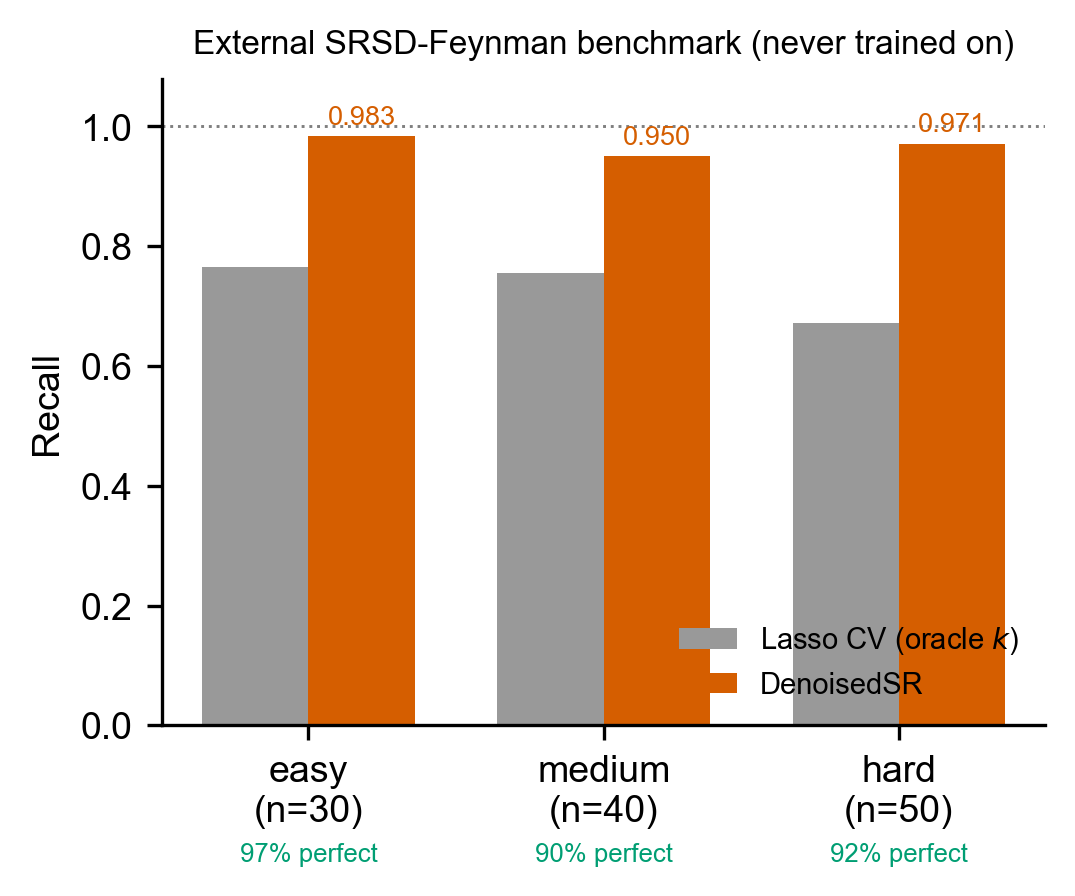
\includegraphics[width=0.55\linewidth]{figures/fig_srsd.png}\hfill
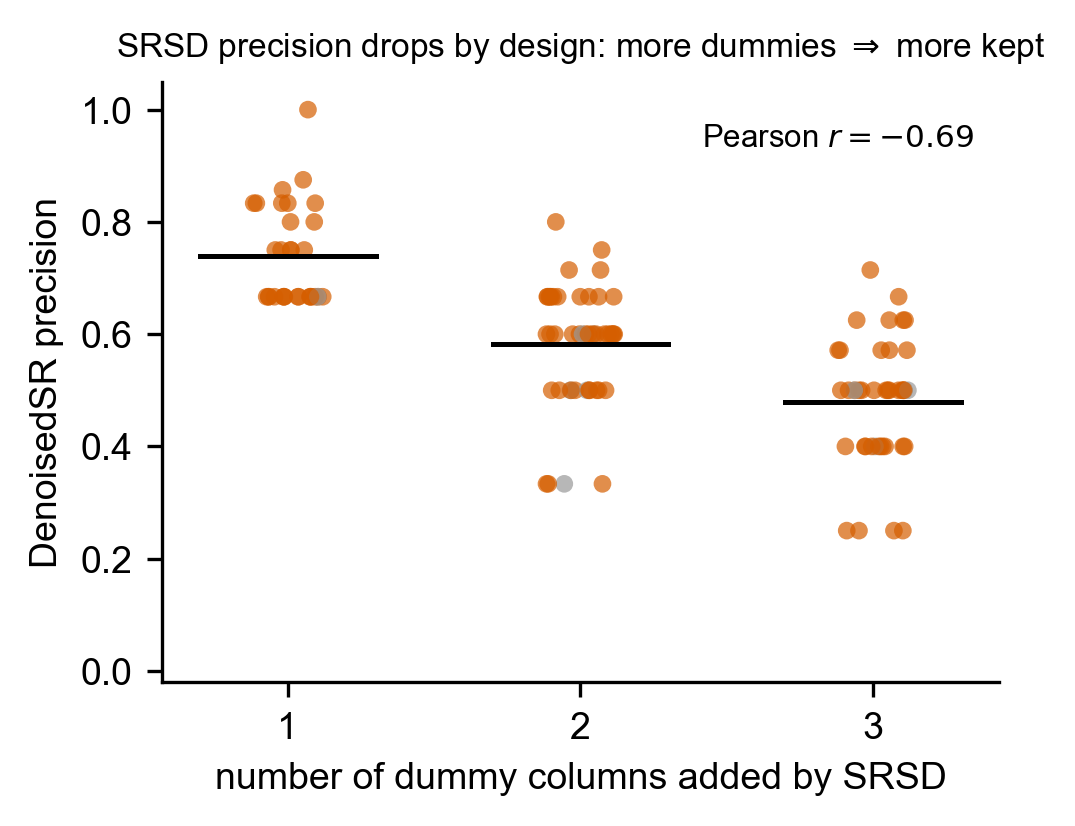
\includegraphics[width=0.42\linewidth]{figures/fig_srsd_precision.png}
\caption{\textbf{Detail on SRSD-Feynman.} \emph{Left}: recall on each SRSD
difficulty split ($30$ easy, $40$ medium, $50$ hard) for DenoisedSR vs.\ Lasso
at oracle top-$k$; DenoisedSR exceeds $0.95$ recall on every split. \emph{Right}:
diagnostic of the apparent precision drop on SRSD ($0.59$ overall). Each marker
is one of the $120$ SRSD tasks (orange = perfect recall, grey = imperfect
recall); horizontal bars show the binned mean precision. Precision falls
monotonically with the number of dummy columns SRSD adds to the task (Pearson
$r=-0.69$) because the front-end at $\tau{=}0.10$ retains physically plausible
dummies rather than discarding them; on tasks with no dummies our precision is
near $1$.}
\label{fig:srsd-detail}
\end{figure}

\

\bibliographystyle{naturemag}
\bibliography{references}

\end{document}
